\documentclass[border=2pt]{standalone}
\usepackage{tikz}
\begin{document}
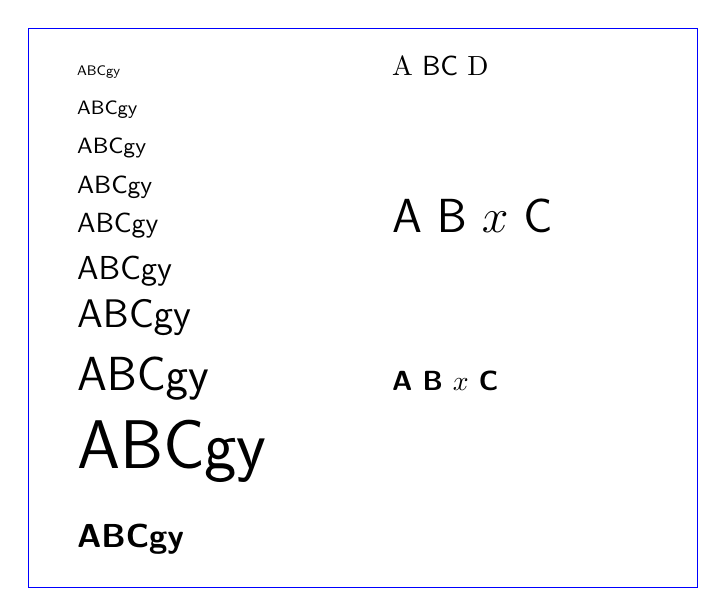
\begin{tikzpicture}
  \draw[blue,line width=.2pt] (-.5,.6) rectangle (8,-6.5);
  \node[anchor=base west,font=\sffamily\tiny] at (0,0) {ABCgy};
  \node[anchor=base west,font=\sffamily\scriptsize] at (0,-.5) {ABCgy};
  \node[anchor=base west,font=\sffamily\footnotesize] at (0,-1) {ABCgy};
  \node[anchor=base west,font=\sffamily\small] at (0,-1.5) {ABCgy};
  \node[anchor=base west,font=\sffamily] at (0,-2) {ABCgy};
  \node[anchor=base west,font=\sffamily\large] at (0,-2.6) {ABCgy};
  \node[anchor=base west,font=\sffamily\Large] at (0,-3.2) {ABCgy};
  \node[anchor=base west,font=\sffamily\LARGE] at (0,-4) {ABCgy};
  \node[anchor=base west,font=\sffamily\Huge] at (0,-5) {ABCgy};
  \node[anchor=base west,font=\sffamily\large\bfseries] at (0,-6) {ABCgy};
  \node[anchor=base west] at (4,0) {A {\sffamily B}\textsf{C} D};
  \node[anchor=base west,text width=3cm,align=flush left,font=\sffamily\LARGE] at (4,-2) {A B $x$ C};
  \node[anchor=base west,text width=3cm,align=flush left,font=\sffamily\bfseries] at (4,-4) {A B $x$ C};
\end{tikzpicture}
\end{document}
